

\chapter{Implementation}
\label{Implementation}
To verify our algorithm we have created a simple, global optimization framework
which enabled us to execute and test all of the algorithms descirbe throughout
this article.

We decided to use Java \cite{java} as a programming language and runtime
environment for this project. 

Using the framework we can find optima of real, mulimodal, multidimensional and
continuous functions. We just need to provide the framework with the concrete
fitness function implementation, domain and by specifing the problem domain.

The framework principle is to separate the interfaces from implementation.
Our API provides interfaces for evolutionary algorithms, fitness assignment
and fitness deterioration, genetic oprators like selection and reproducion,
phenotype, clustering algorithms and many more. This makes it compact,
extensible and easy to indroduce new implementations.
For the detailed description of the classes and interfaces see subsection
'Implementation in Java'.  

\section{Architecture}

The project consists of six main packages, which communicates with the
others through clearly specified interfaces and together constitute a
complete, lightweight framework for testing and execution of the global 
optimization algorithms especially the evolutionary algorithms.
\begin{itemize}
  \item \textit{Algorithm module}
  \item \textit{Clustering module}
  \item \textit{Fitness deterioration module}
  \item \textit{Evolutionary Algorithms module}
  \item \textit{Printing Modul}
  \item \textit{Statistics Utils}
\end{itemize}

\section{Implementation in Java}
clean structure, good test coverage, 
modular architercture, extensible,
\lstinputlisting{test-context.xml}

\subsection{Technologies}
\begin{itemize}
  \item Spring \cite{spring} - application framework
  \item Maven \cite{maven} - project management and build automation
  \item Mockito \cite{mockito} - testing framework 
  \item JAMA \cite{jama} - linear algebra package
\end{itemize}
Spring, Maven, JUnit, Mockito, JAMA, TDD approach

\subsection{Diagrams}
class diagrams, sequence diagrams

Below you may find class diagrams for each of the module implemented in our
framework. It shows a general overview of the structure of a system: used
classes, their attributes, operations and the relationships between the classes.


\begin{figure}
  \centering
  \fbox{
    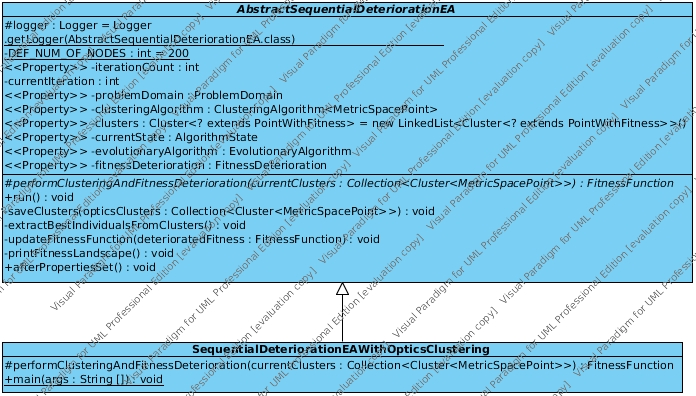
\includegraphics[scale=0.5]{ClassDiagrams/algorithm.jpg}
  }
  \caption{Main algorithm package}
  \label{alg}
\end{figure}

\begin{figure}
  \centering
  \fbox{
    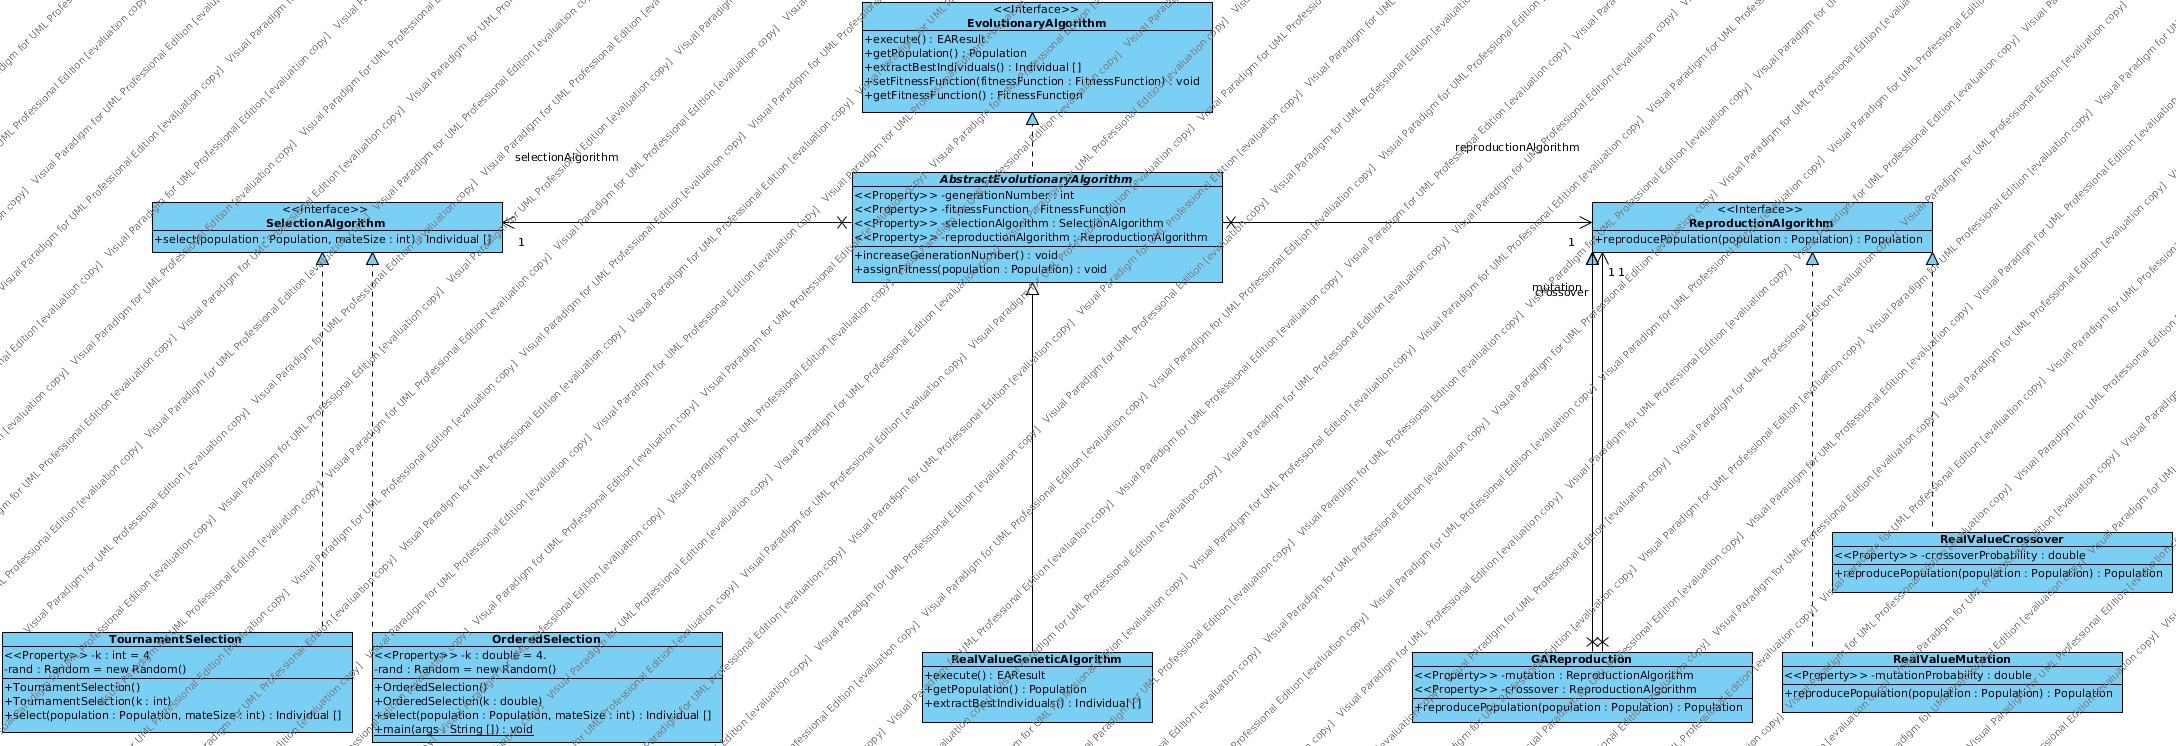
\includegraphics[scale=0.3, angle=90]{ClassDiagrams/EA.jpg}
  }
  \caption{Evolutionary algorithms package}
  \label{ea}
\end{figure}

\begin{figure}
  \centering
  \fbox{
    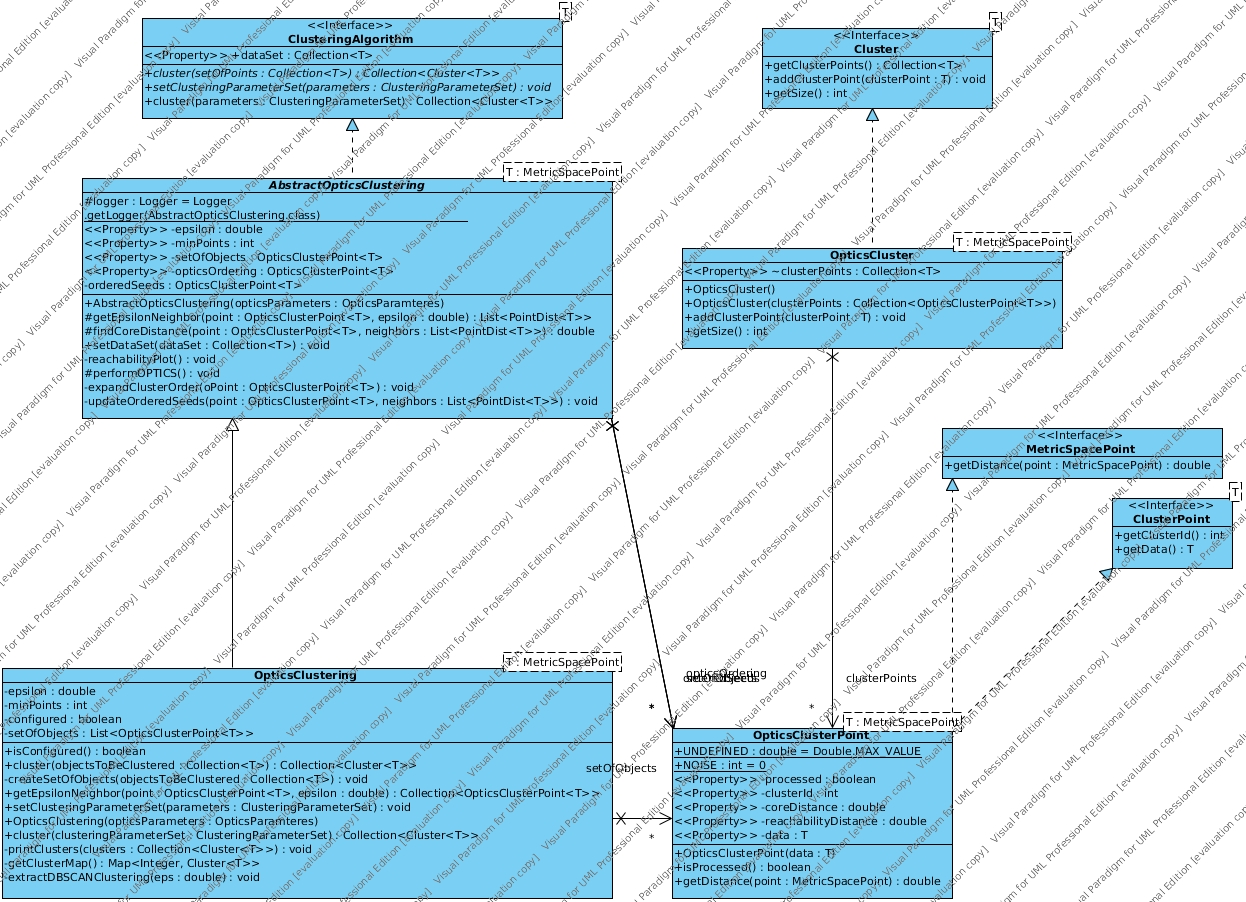
\includegraphics[scale=0.3, angle=90]{ClassDiagrams/clustering.jpg}
  }
  \caption{Clustering package}
  \label{optics}
\end{figure}

\begin{figure}
  \centering
  \fbox{
    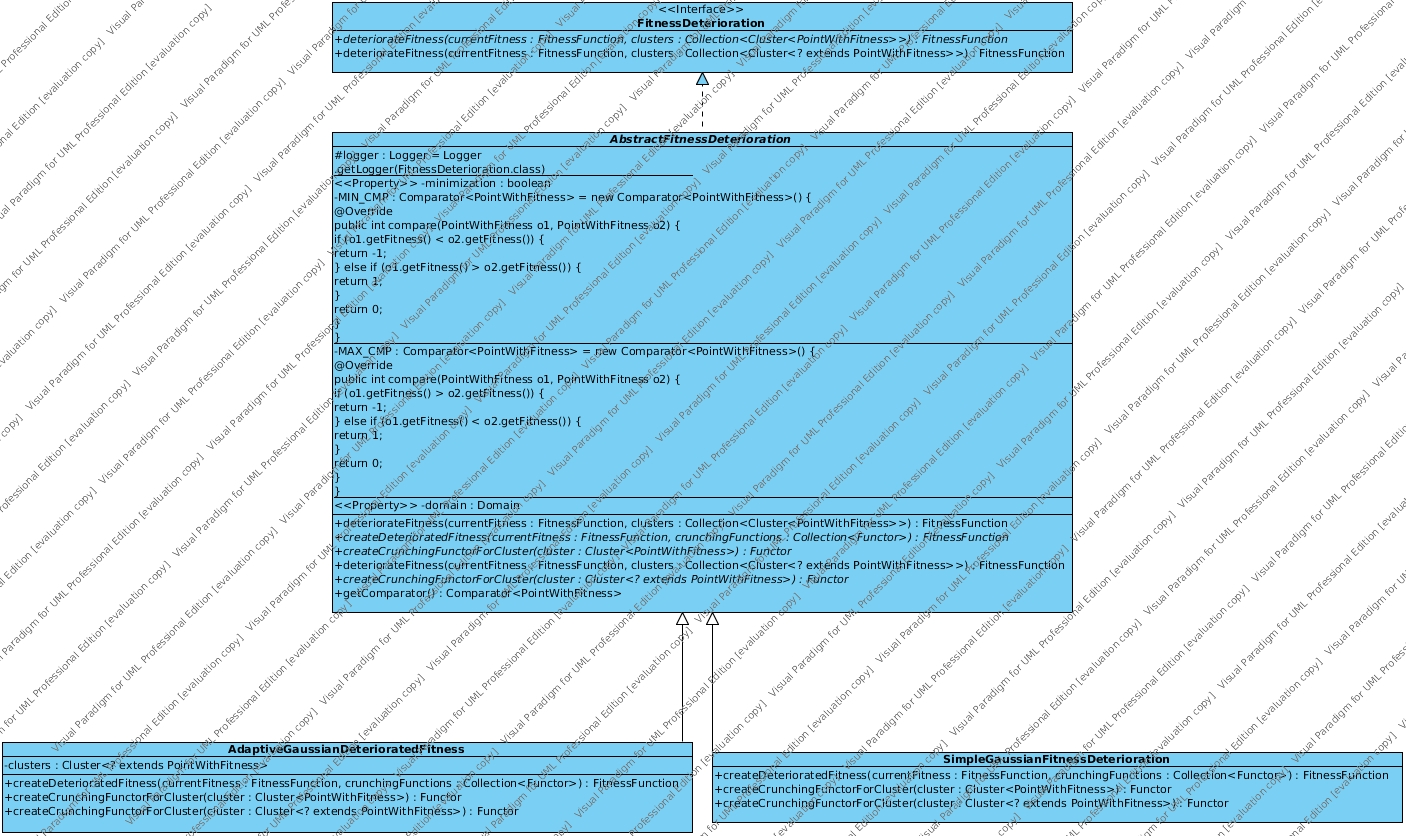
\includegraphics[scale=0.3, angle=90]{ClassDiagrams/deterioration.jpg}
  }
  \caption{Fitness deterioration package}
  \label{fitdet}
\end{figure}

\begin{figure}
  \centering
  \fbox{
    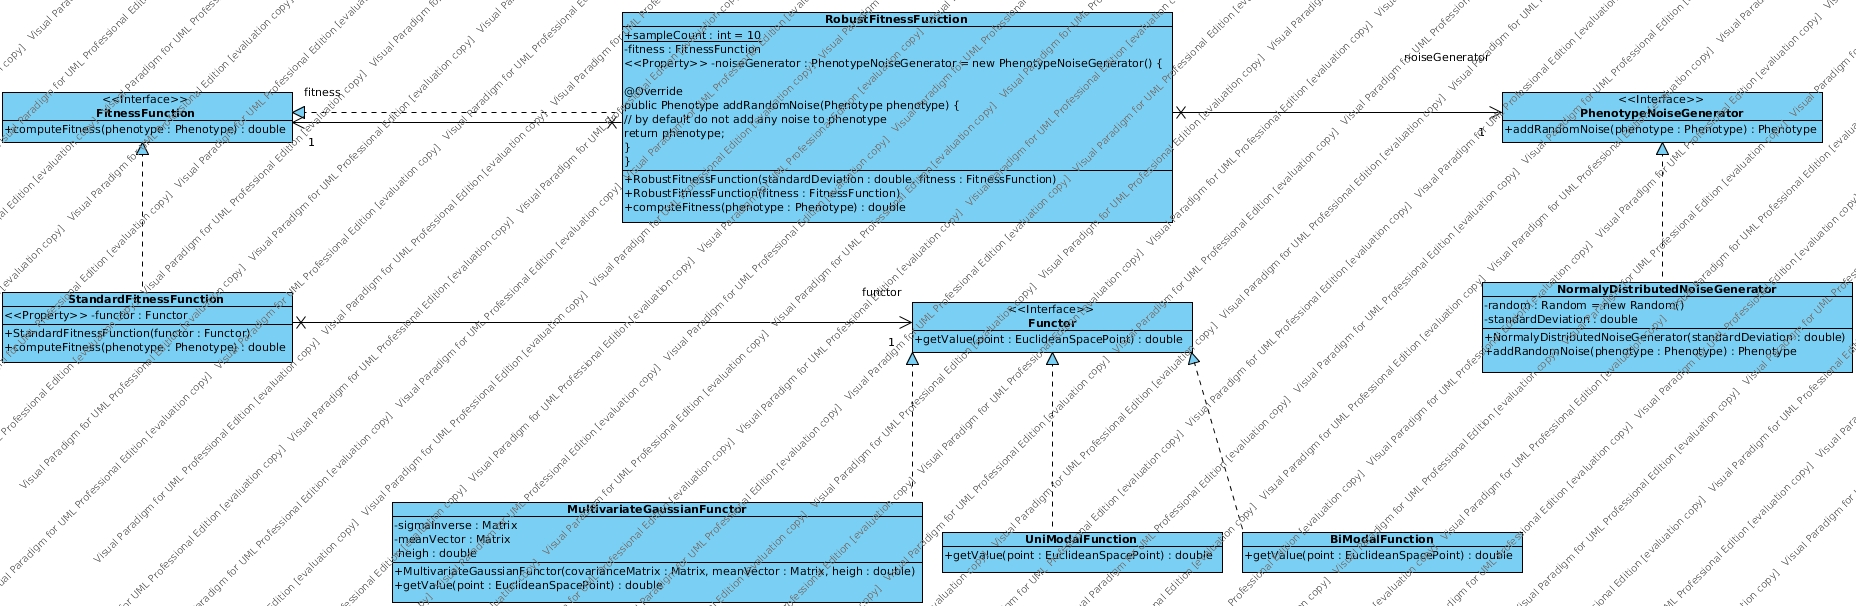
\includegraphics[scale=0.3, angle=90]{ClassDiagrams/fitness.jpg}
  }
  \caption{Fitness and functors package}
  \label{ea}
\end{figure}

\begin{figure}
  \centering
  \fbox{
    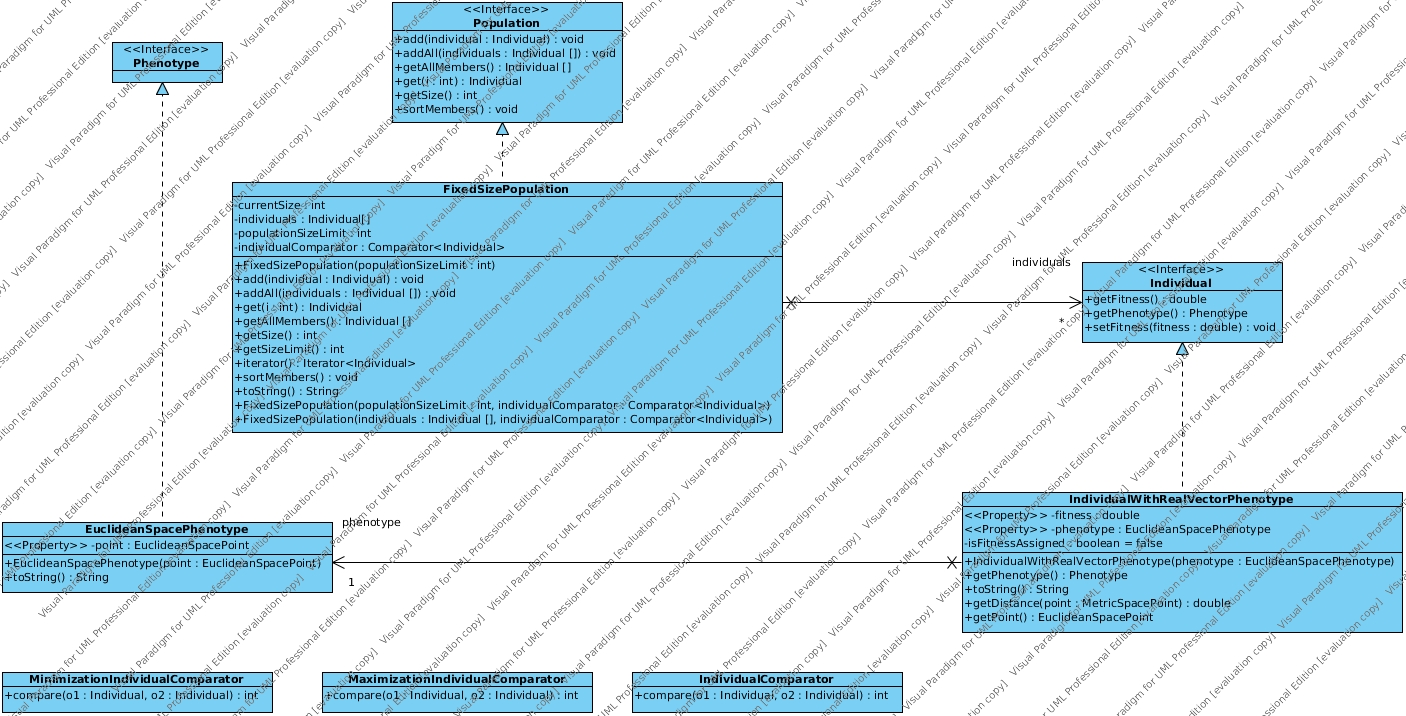
\includegraphics[scale=0.3, angle=90]{ClassDiagrams/population.jpg}
  }
  \caption{Population package}
  \label{ea}
\end{figure}